We are interested here in analyzing the performances obtained per speaker, according to their characteristics, for instance in terms of speech turns etc. As the speech turns properties depend on the show in which the speaker appears, one speaker in one show is considered as the unit of analysis, the so-called $SpkShow$. One speaker appearing in 2 different videos is considered as 2 distinct $SpkShow$.

The test corpus contains about 10 hours of annotated contents, on 62 different videos, totalizing 477 non-anonymous different $SpkShow$.

In the analysis, we adopt the point of view of the references: for each $SpkShow_i$ in the reference is computed a performance measure of the biometric system, defined as the F-measure of the detection of $SpkShow_i$. More precisely, considering the definition given in \ref{notation}, Precision and Recall can be computed for each $SpkShow_i$:
\begin{itemize}
\item $Precision_i=\frac{T^{corr}_i}{T^{test}_i}$
\item $Recall_i=\frac{T^{corr}_i}{T^{ref}_i}$
\item $Fm_i=\frac{2*Precision_i*Recall_i}{Precision_i+Recall_i}$
\end{itemize} 

Thus, $Fm_i=0$ means that $SpkShow_i$ was never correctly identified, whereas $Fm_i=1$ means that $SpkShow_i$ is perfectly identified, without miss detection nor false alarm.

The table \ref{table-spkshow-perf} shows the average $Fm$ per $SpkShow$ for the different systems.
\begin{table*}[t]
\begin{center}
\begin{tabular}{r||c|c|c}
& Percol & Qcompere & Soda \\\hline\hline
average $Fm$ & 0.361 & 0.381 & 0.351\\\hline
average $Fm$ for in dictionary speakers & 0.628 & 0.684 & 0.619\\\hline
\#$SpkShow$ out of dictionary & 200 & 209 & 204 \\\hline
\#$SpkShow$ in dictionary & 277& 268 & 273\\\hline
\#$SpkShow$ in dictionary, with $Fm=0$ & 79 & 63 & 86\\\hline
\end{tabular}
\caption{Average system performances per $SpkShow$}
\label{table-spkshow-perf}
\end{center}
\end{table*}

From the table we can notice the important number of $SpkShow$ which are not in the dictionary of the system, about 40\% for each system. As they don't have any model, they obviously cannot be identified, leading to an average global $Fm$ rather poor. More interestingly, the number of $SpkShow$ which are actually in the dictionary and which are not recognised at all, is not negligeable: their represent between 23.5\% to 31.5\% of the in-dictionary $SpkShow$, according to the systems.


The flgure \ref{PQS} plot the distribution of all the $SpkShow$ in the system dictionaries, according their performance $Fm$, for the different systems. Foreach $Spkshow$, the average performance and the maximal performance obtained across systems are computed, and the corresponding distribution are also plotted. We can see from this figure that the average performance (from 61.9\% to 68.9\% according to the systems) presented in table\ref{table-spkshow-perf} is not at all representative of the performances obtained foreach $SpkShow$: speakers are either not recognized or well recognized. Indeed, if we compute the average performance for $SpkShow$ which have $Fm \neq 0$, the average $Fm$ grows to 87.9\% for PERCOL, 89.5\% for QCompere and 90.3\% for SODA. 

\begin{figure}[!h]
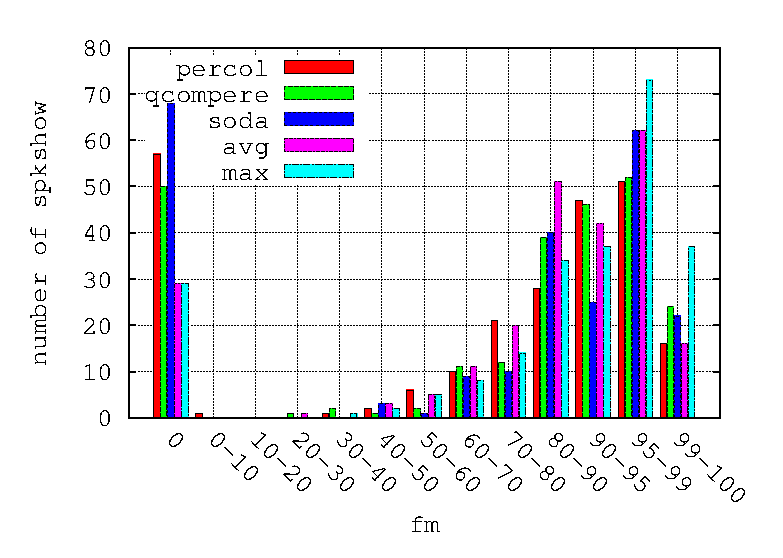
\includegraphics[scale=0.6]{PQS-mono-model.eps}
\caption{$spkShow$ performance distribution, for each system}
\label{PQS}
\end{figure}

To evaluate the impact of the automatic speaker diarization, we also perform the speaker analysis performance, for systems applied on reference speaker diarization. Results for systems PERCOL and SODA are plotted in figures \ref{soda-autoref} and \ref{percol-autoref}.  

\begin{figure}[!h]
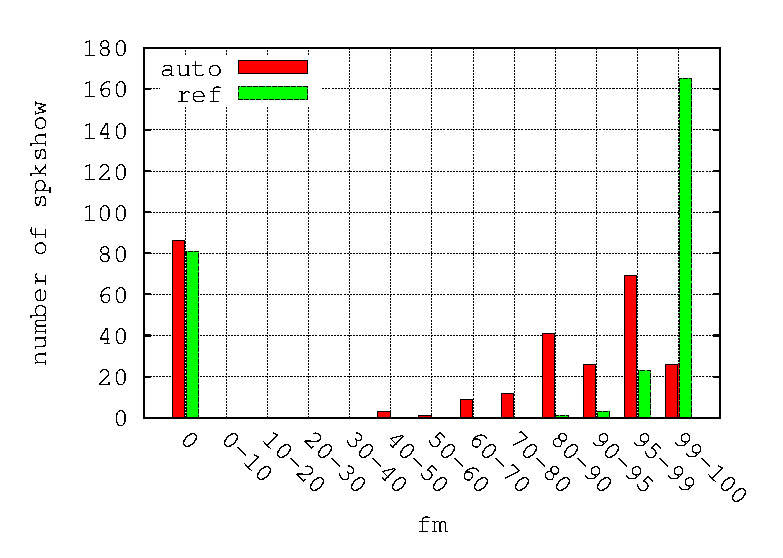
\includegraphics[scale=0.6]{SODA.eps}
\caption{$spkShow$ performance distribution, for SODA system, with reference and automatic speaker diarization}
\label{soda-autoref}
\end{figure}

\begin{figure}[!h]
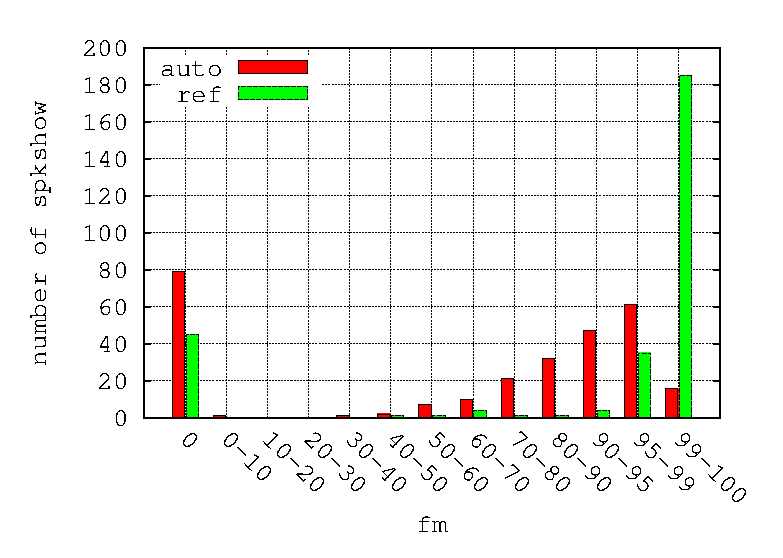
\includegraphics[scale=0.6]{PERCOL.eps}
\caption{$spkShow$ performance distribution, for PERCOL system, with reference and automatic speaker diarization}
\label{percol-autoref}
\end{figure}


